\documentclass[12pt,a4paper,oneside]{article}
\usepackage[spanish,activeacute]{babel}
\usepackage[utf8]{inputenc}
\usepackage[left = 2.5cm, top = 2cm, right = 2.5cm, bottom = 2cm]{geometry}
\usepackage{graphicx}

\spanishdecimal{.}

\newpage\pagenumbering{arabic}
\setcounter{page}{1}

\renewcommand{\baselinestretch}{1}
\begin{document}

\part*{Anexo X}

\subsection*{Gráficos de la \textit{aggregation rule}}
\vspace*{1\baselineskip}
\begin{figure} [h]
    \centering
    \centerline{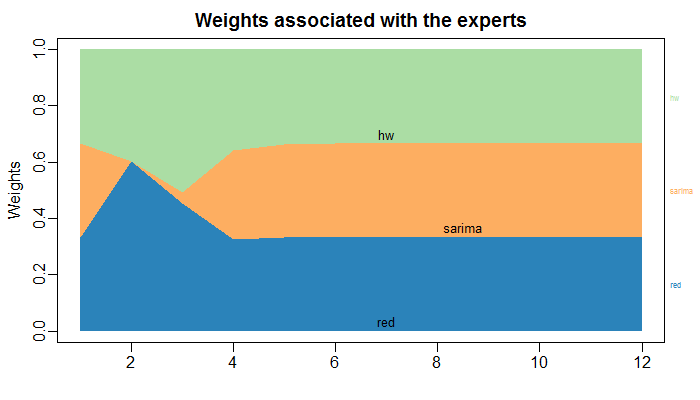
\includegraphics[scale = 0.7]{Images/1.png}}
    \caption{Evolución de las ponderaciones}
    \label{red}
\end{figure}
\vspace*{3\baselineskip}
\vspace*{3\baselineskip}
\begin{figure} [h]
    \centering
    \centerline{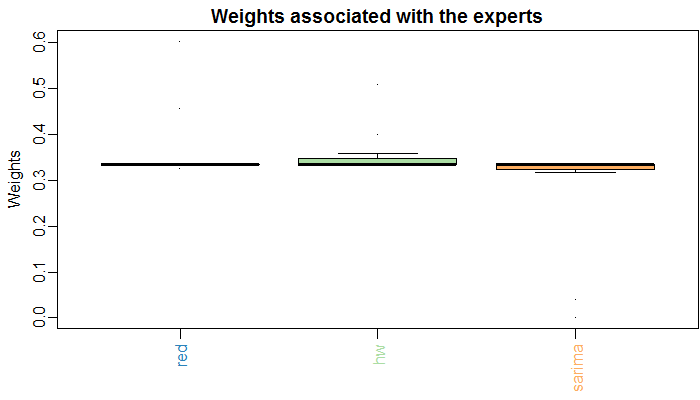
\includegraphics[scale = 0.7]{Images/2.png}}
    \caption{Box-plot de las ponderaciones}
    \label{red}
\end{figure}
\begin{figure} [h]
    \centering
    \centerline{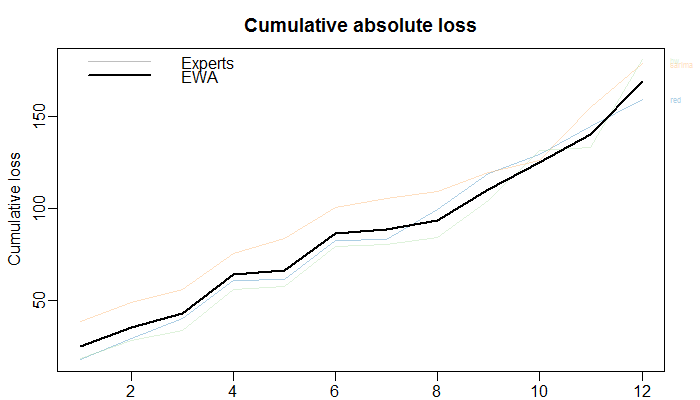
\includegraphics[scale = 0.7]{Images/3.png}}
    \caption{MAE acumulado durante la estimación de las ponderaciones}
    \label{red}
\end{figure}
\vspace*{3\baselineskip}
\vspace*{3\baselineskip}
\vspace*{3\baselineskip}
\begin{figure} [h]
    \centering
    \centerline{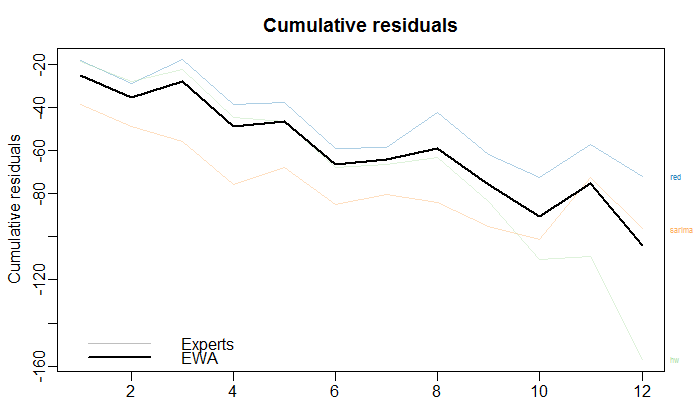
\includegraphics[scale = 0.7]{Images/4.png}}
    \caption{Residuos acumulados}
    \label{red}
\end{figure}
\begin{figure} [h]
    \centering
    \centerline{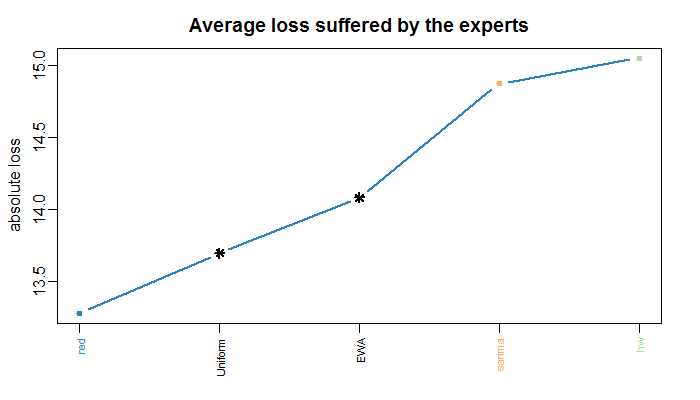
\includegraphics[scale = 0.7]{Images/5.png}}
    \caption{MAE de los modelos y las combinaciones}
    \label{red}
\end{figure}
\vspace*{3\baselineskip}
\vspace*{3\baselineskip}
\vspace*{3\baselineskip}
\begin{figure} [h]
    \centering
    \centerline{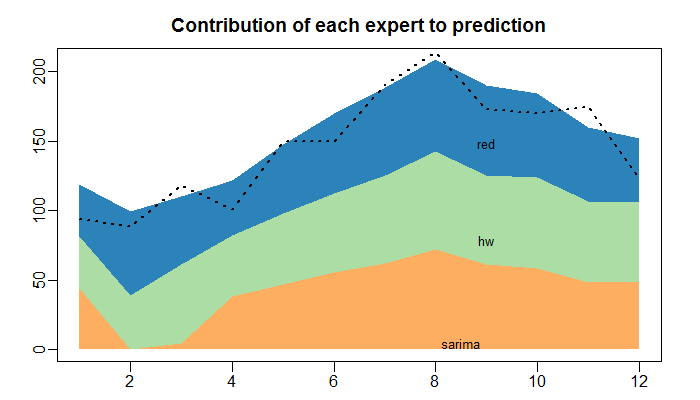
\includegraphics[scale = 0.7]{Images/6.png}}
    \caption{Contribución de cada modelo a la predicción final}
    \label{red}
\end{figure}
\vspace*{3\baselineskip}

\end{document}
